\documentclass[a4paper,12pt]{article}
\usepackage{graphicx}
\usepackage[left=30mm, right=30mm, top=30mm, bottom=35mm]{geometry}
\usepackage{amsmath}
\usepackage{siunitx}
\usepackage{fancyhdr}
\usepackage{url}
\pagestyle{fancy}
%-------------------------------------------------------------------------------
\lhead{\textbf{Spring 2019}}
\rhead{\textbf{CE394M Advanced Analysis in Geotechnical Engineering}}
\cfoot{\thepage}
%-------------------------------------------------------------------------------

\begin{document}
\begin{centering}
	\textbf{
		Project 1: Finite Element modeling of a propped excavation in clay\\
		Assigned: 1st April 2019\\
		Due: 19th April 2019\\
	}
\end{centering}

\vspace{1em}

\textbf{Note: }\textit{This is a group project and your results should be submitted 
	individually in a report format.}

You may obtain access to Plaxis through a Virtual Desktop.  Information about gaining access can be found at \url{ http://caee.utexas.edu/students/itss/43-students/it/386-virtualdesktops}.  

A \SI{70}{\meter} wide excavation is to be dug in uniform stages through 
\SI{4}{\meter} of silty-sand fill into normally consolidated clay that 
extends to a great depth. The excavation will be supported by a diaphragm wall 
from the ground surface (\SI{+21.5}{\meter}~OD) to a base elevation of 
\SI{-5.0}{\meter}~OD and a single row of props at an elevation of 
\SI{+20}{\meter}~OD.  During excavation, a pressure 
load of \SI{5}{\kilo\pascal} will act at the ground surface within 
\SI{25}{\meter} of the wall.  The geometry and material parameters for the 
problem are presented below:

\begin{figure}[h]
	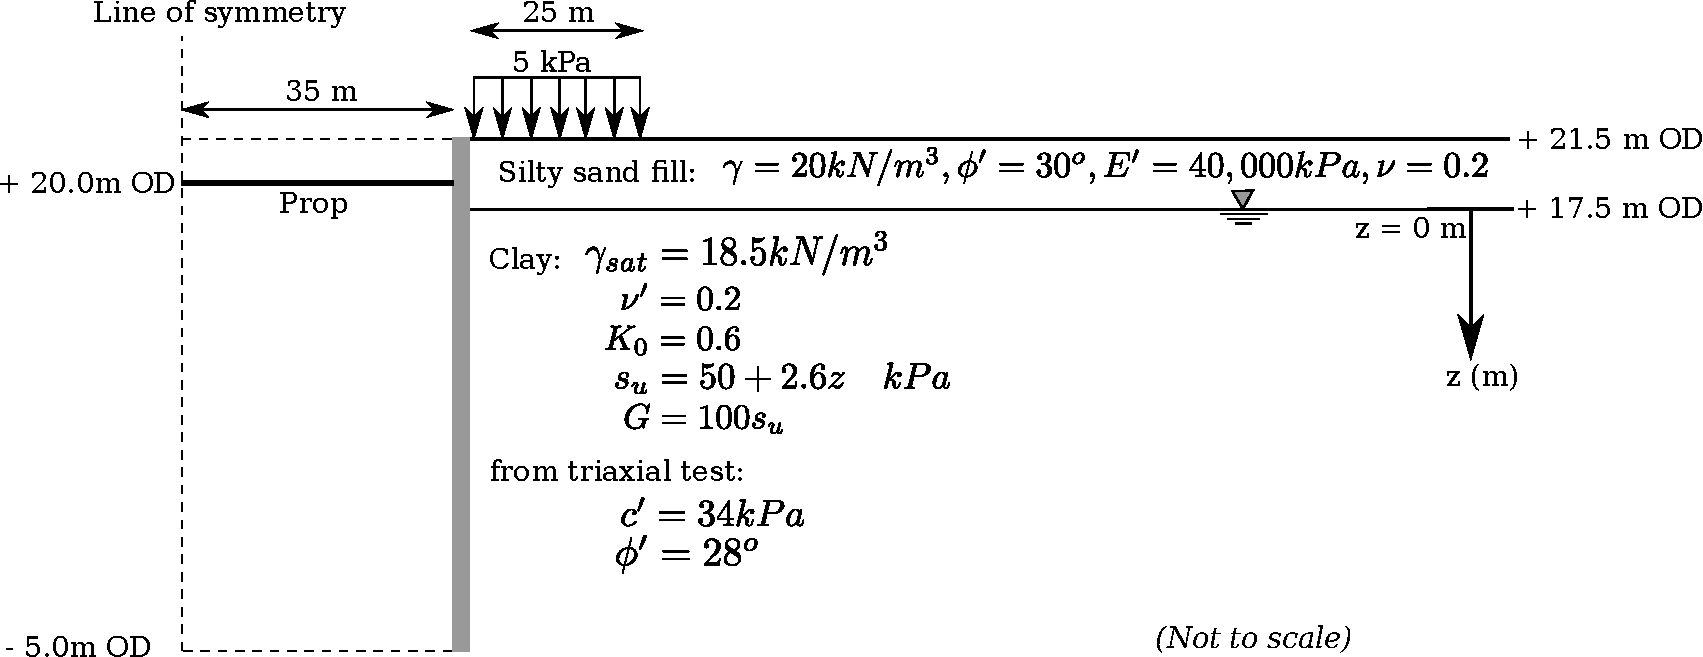
\includegraphics[width=\textwidth]{Problem.pdf}
\end{figure}

\begin{center}
	\textbf{Wall Parameters:} EA = $7.5\times 10^6$ kN/m; EI = 1.0$\times10^6$ 
	kN/m$^2$/m; \\ w = 10 kN/m/m; $\nu$=0.15 \\
	Prop Parameters: EA=$2.0\times10^6$ kN/m; $L_{spacing}$ = 5 m.
\end{center}


\begin{enumerate}
	\item
	Perform a plane strain finite element analysis in PLAXIS using the Mohr--Coulomb model without dilation and total stress method. Model the wall using beam and interface elements and the prop using a fixed end anchor. Assume the wall and props are perfectly elastic.
	
	\textit{Hint: Perform a ``drained'' analysis with no water, but specify undrained material parameters in the clay (note that the Poisson's Ratio cannot be set to $\nu$=0.5 so use $\nu$=0.495 instead).}
	\begin{enumerate}
		\item
		Determine the excavation depth at which some material points will begin to exceed the Mohr--Coulomb strength criterion in the clay.
		\item
		Determine the maximum excavation depth at which the horizontal wall movements will not exceed 100mm.
		\item
		When the excavation depth reaches +7.5m:
		\begin{enumerate}
			\item
			Plot the total displacement and mean total (or effective) stress contours,
			\item
			Plot horizontal displacement and bending moment along the wall,
			\item
			Record the prop forces.
		\end{enumerate}
		\item
		Determine the maximum excavation depth at which the system will collapse. Plot the plastic points at this depth and identify the failure mechanism.
	\end{enumerate}
	\item
	Repeat part 1(a -- c) using the effective stress method and the parameters determined from triaxial testing.
	\item
	Repeat part 1(a -- c) using the effective stress method and equivalent Mohr Coulomb parameters derived from the shear strength profile.
	
	\textit{Hint: Determine effective stress parameters from the shear strength 
		profile by constructing Mohr's Circles.}
	
	\item
	Discuss the role of tension cut-off in finite element simulations and give an example of a situation where this might be important. Does tension cut--off play an important role for this propped excavation?
	\item
	Compare and contrast the three different analysis methods, paying particular attention to the prop forces and depth--displacement curves. What are the advantages and disadvantages of each method?
	\item
	Pore pressures can only be generated using effective stress methods. Are the pore pressures computed using Mohr--Coulomb reasonable? How might the computed pore pressures (and shear strengths) be different if a more advanced soil model was used?
\end{enumerate}
\end{document}

